\definecolor{chinese}{rgb}{0.58, 0.77, 0.45} %chinese #green
%english #blue
%french #red
%german #yellow
%japanese #grey
%russian #orange
%spanish #magenta


\begin{figure}
\centering

        \begin{tikzpicture}
        \begin{scope}[xshift=1.5cm]
            \node[anchor=south west,inner sep=0] (image) at (0,0)
            {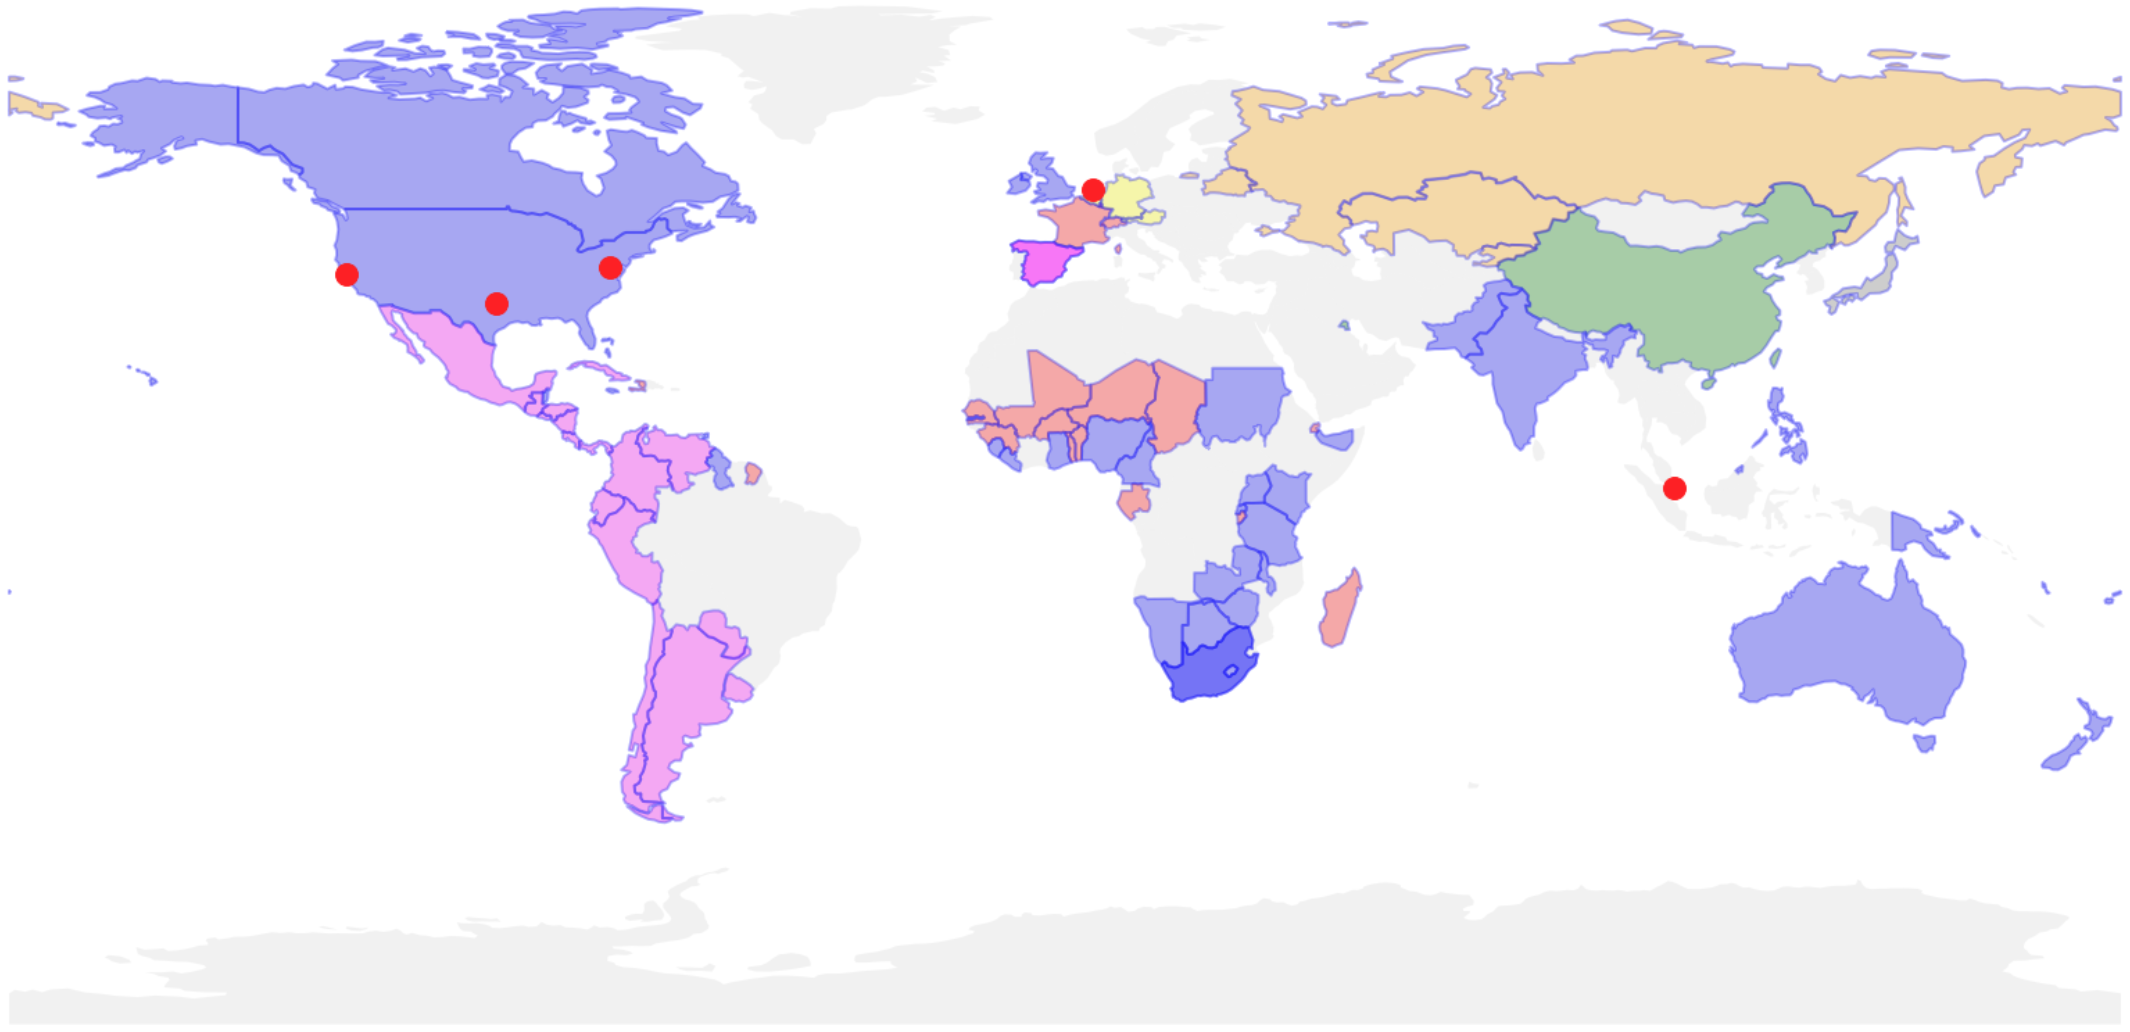
\includegraphics[width=1\textwidth]{embodied_cost_model/images/world_language_map.png}};
        \end{scope}
        \node [anchor=center] (chinese) at (2,-.6) {\small{Chinese}};
        \filldraw[outer color=chinese, inner color=chinese] (1.8,-.4) rectangle (2.2,0); % cpu
            
        \end{tikzpicture}

\caption[Source country of language and DC locations]{Source country of language and DC locations map.}
\label{image:world_language_map}
\end{figure}